%% ==========================================================================
%%  PACR -- Patient-Aware Agentic Cyber-Resilience for the IoMT
%%  Elsevier single-column (elsarticle, preprint, 12pt).  Self-contained:
%%  figures are TikZ/pgfplots with the measured data embedded, and the
%%  bibliography is inline, so it compiles as one file (Overleaf: pdfLaTeX).
%%
%%  Search for "TODO" before submitting: author names/affiliation, the target
%%  journal's own template (change only the \documentclass line and the
%%  frontmatter block), and the "VERIFY" notes on the related-work table.
%% ==========================================================================
\documentclass[preprint,12pt]{elsarticle}

\usepackage[utf8]{inputenc}
\usepackage{amsmath,amssymb}
\usepackage{booktabs,array,multirow,tabularx}
\usepackage{graphicx}
\usepackage{xcolor}
\usepackage{microtype}
\usepackage{algorithm}
\usepackage{algpseudocode}
\usepackage{tikz}
\usetikzlibrary{arrows.meta,positioning,shapes.geometric,fit,backgrounds,calc}
\usepackage{pgfplots}
\pgfplotsset{compat=1.18}
\usepackage[hidelinks]{hyperref}

\biboptions{numbers,sort&compress}

% ---- colours used by every figure -----------------------------------------
\definecolor{pacrblue}{RGB}{31,94,168}
\definecolor{pacramber}{RGB}{214,148,24}
\definecolor{pacrgrey}{RGB}{110,110,110}
\definecolor{pacrred}{RGB}{190,52,52}
\definecolor{pacrgreen}{RGB}{46,125,50}

% ---- small helpers ---------------------------------------------------------
\newcommand{\pacr}{\textsc{Pacr}}
\newcommand{\cic}{CICIoMT2024}
\newcolumntype{L}[1]{>{\raggedright\arraybackslash}p{#1}}
\newcolumntype{C}[1]{>{\centering\arraybackslash}p{#1}}
\renewcommand{\arraystretch}{1.15}
\setlength{\tabcolsep}{4pt}

\journal{TODO: target journal}

\begin{document}

\begin{frontmatter}

\title{Patient-Aware Agentic Cyber-Resilience for the Internet of Medical Things:
Guarded LLM Incident Response with Blockchain Provenance}

% TODO: replace with the real author list and affiliations.
\author[aff1]{Darshan K\corref{cor1}}
\ead{kdarshan.crg@gmail.com}
\author[aff1]{TODO: co-author / faculty guide}
\cortext[cor1]{Corresponding author}
\address[aff1]{Department of Electrical and Electronics Engineering, Amrita School of Engineering, Coimbatore, India}  % TODO: check department / school

\begin{abstract}
Hospitals depend on networked medical devices, yet an automated cyber response can itself harm a patient: isolating an attacked ventilator stops breathing support. Existing Internet of Medical Things (IoMT) detectors end at classification, and language-model incident-response agents give no guarantee against wrong or manipulated output. We propose \pacr, a four-phase, patient-aware cyber-resilience framework. It combines an XGBoost detector with calibrated confidence, five language-model agents treated as untrusted components, deterministic grounding guards, rule-based risk and policy engines that require a human for severe actions on patient-dependent devices, and a Hyperledger Fabric ledger for tamper-evident provenance. On the full CICIoMT2024 test split (1,614,182 flows) the detector reaches 99.52\% 19-class accuracy and 99.97\% attack detection. The full system takes 0.00\% unsafe autonomous actions, against 99.72\% for a fixed-response baseline. Under ten injected agent faults the guards reduce unsafe actions from two to zero, and the ledger detected every tested tampering.
\end{abstract}

\begin{keyword}
Internet of Medical Things \sep cyber-resilience \sep agentic AI \sep large language models \sep patient safety \sep Hyperledger Fabric \sep CICIoMT2024
\end{keyword}

\end{frontmatter}

%% ==========================================================================
\section{Introduction}
\label{sec:intro}

\paragraph{Broad area.}
The Internet of Medical Things (IoMT) connects infusion pumps, patient monitors, ventilators and imaging equipment to hospital networks, and with that connectivity comes a large attack surface. Research on IoMT security has produced a large body of intrusion-detection work, which recent reviews organise by method, dataset and evaluation metric~\cite{naghib2025}. The CICIoMT2024 benchmark~\cite{dadkhah2024}, collected from a testbed of IoMT devices under attack over several protocols, has become a common test bed. Detectors built on it now report high accuracy: an enhanced LSTM called L2D2 reaches 98\% over 19 classes~\cite{akar2025}, a reinforcement-learning hybrid reaches 0.9958 binary accuracy~\cite{shaikh2025}, and an interpretable XGBoost fusion reaches 0.97~\cite{hafid2025}.

\paragraph{Objective.}
The objective of this work is to move from \emph{detecting} an attack on a medical device to \emph{responding} to it safely. A response is safe only if it does not harm the patient who depends on the device, and it is useful only if it can be explained and audited afterwards.

\paragraph{Problem statement.}
In a clinical network the most secure response is not always the safest one. A fixed playbook that isolates any device under attack will, on a ventilator, remove breathing support to stop a network flood. Language-model agents have recently been proposed to automate incident response~\cite{lin2025,gao2026}, but a model can be wrong, can be misled by text inside the traffic it reads, and can claim that a device has recovered while the attacker is still active. Blockchain has been proposed to protect health records and evidence~\cite{hasnain2023,pelekoudas2023}, yet it is rarely measured on a real ledger together with detection and response. The open problem is therefore: given IoMT traffic and a registry of device criticality, choose an automated response whose risk to a patient-dependent device is controlled \emph{by construction}, whatever an AI component says, and keep a tamper-evident record of every step.

\paragraph{Related directions.}
Closely related work on healthcare blockchains from our own institution combines smart contracts with encryption for medical data sharing~\cite{vidhya2023} and builds a smart-contract blockchain for a healthcare IoT network~\cite{mukhopadhyay2021}, while cyber-physical work applies machine learning to attack classification and anomaly detection in power systems~\cite{pranav2026,vignes2025}. These share our concern with trustworthy automation in safety-critical infrastructure, but none of them gates an automated response on the clinical state of a device.

\paragraph{Contributions.}
This paper makes the following contributions.
\begin{enumerate}
  \item \textbf{A patient-aware response architecture.} \pacr{} separates reasoning (five language-model agents) from decision (deterministic Risk and Policy engines), so that no agent can by itself cause a disruptive action on a high-stakes device.
  \item \textbf{Deterministic grounding guards.} Three guards treat agent output as untrusted: the device registry overrides a model's clinical-context claim, a recovery claim is overridden if attack traffic continues, and an answer about the wrong incident is rejected.
  \item \textbf{A calibrated confidence gate.} Temperature-scaled detector confidence, with a threshold chosen on held-out validation data and scored once on test, reduces unnecessary autonomous isolation on false alarms.
  \item \textbf{Blockchain provenance measured on a real network.} Incident, decision, approval, response and recovery are written to a Hyperledger Fabric ledger; integrity, tamper evidence, latency and concurrency are measured on a real two-organisation network.
  \item \textbf{A safety-focused evaluation.} On all 1,614,182 official CICIoMT2024 test flows we report unsafe-autonomous-action and unnecessary-isolation rates against baselines and ablations, and a fault-injection study of the agentic layer with the guards on and off.
\end{enumerate}

\paragraph{Organisation of the paper.}
Section~\ref{sec:lit} reviews ten related works and states the identified gaps. Section~\ref{sec:method} presents the proposed framework, its four phases and algorithms. Section~\ref{sec:results} gives the experimental setup, dataset and results. Section~\ref{sec:comparison} compares \pacr{} with existing work. Section~\ref{sec:conclusion} concludes with directions for future research.

%% ==========================================================================
\section{Literature review}
\label{sec:lit}

Table~\ref{tab:lit} summarises ten recent works that are close to ours in one of three respects: IoMT intrusion detection, blockchain for healthcare or forensic evidence, and language-model agents for incident response. For each we state the algorithm, its advantage, and its drawback \emph{with respect to our objective of safe, auditable automated response}. The drawbacks are therefore not criticisms of the works' own aims.

% VERIFY: the "Advantage" and "Drawback" cells were written from each paper's
% abstract / title and the figures quoted there. Re-read each paper's full text
% before submission and adjust any drawback that its authors do address.
\begin{table}[htbp]
\centering
\caption{Ten related works (2023--2026): algorithm, advantage and drawback relative to this work.}
\label{tab:lit}
\footnotesize
\begin{tabular}{@{}C{0.8cm}L{2.9cm}L{3.0cm}L{3.1cm}L{2.9cm}@{}}
\toprule
Ref. & Algorithm / approach & Advantage & Drawback & Gap for our problem \\
\midrule
\cite{akar2025} & Enhanced LSTM (L2D2) on CICIoMT2024, 19 classes. & 98\% accuracy on the real multi-class benchmark. & Detection only; no response, clinical context or provenance. & Classification stops before the decision that affects a patient. \\
\cite{shaikh2025} & CNN-LSTM features with DQN and PPO decision learners; mutual-information feature selection; CICIoMT2024. & 0.9958 binary accuracy; learned decision policy. & 18-class accuracy only 0.7773, so attack type is uncertain; decisions are about classification, not device impact. & Learned policies are not gated by what the response does to the device. \\
\cite{hafid2025} & Tuned XGBoost with logistic-regression late fusion and SHAP; cost-aware; CIC IoMT 2024. & Interpretable; fusion cut false negatives from 361 to 213. & Cost is a generic security cost; no patient impact; no automated response. & Interpretability of detection, not of response safety. \\
\cite{alsolami2024} & Stacking, bagging and boosting of random forest and SVM; WUSTL-EHMS-2020. & 98.88\% accuracy with stacking; uses patient-biometric features. & One dataset, as the authors note; detection only. & No link from detection to a safe action. \\
\cite{abdelhaq2026} & Soft-voting XGBoost and two SVMs, PCA features; WUSTL-EHMS-2020, validated on TON-IoT and CICIDS 2017. & 98.04\% accuracy; cross-dataset validation. & Detection only; no response or clinical gating. & Same gap: no action layer. \\
\cite{hasnain2023} & Systematic review of Hyperledger Fabric for health-record security (57 studies). & Collects the privacy, integrity and traceability benefits of Fabric. & A review: no implementation and no incident response. & Evidence of need, not a measured system. \\
\cite{pelekoudas2023} & Prototype Hyperledger Fabric security architecture for IoMT health monitoring. & A real Fabric prototype aimed at IoMT. & Scope is the monitoring system's data security, not an automated response decision. & Ledger not tied to detector, agents or response gating. \\
\cite{xiao2024} & Blockchain digital-forensics scheme for industrial IoT: smart contracts, token access control, batch consensus. & Tamper-proof, non-repudiable evidence chain; faster than DPoS in simulation. & Industrial setting; evaluated in simulation; no clinical safety notion. & No patient-dependent action policy. \\
\cite{lin2025} & IRCopilot: four cooperating LLM sessions that mirror incident-response phases (preprint). & Role split reduces context loss and hallucination. & No deterministic guard on model output; not medical; no clinical gating. & An unguarded agent can still recommend a harmful action. \\
\cite{gao2026} & Fine-tuned 14B LLM with perception, reasoning, planning and action, plus in-context adaptation (preprint). & Recovery up to 23\% faster than frontier models. & Optimises recovery time; patient harm not modelled; a five-action plan takes about 20 minutes on an A100. & Speed is not the binding constraint when a patient depends on the device. \\
\bottomrule
\end{tabular}
\end{table}

Two further observations come from this review and from the closely related institutional work cited in Section~\ref{sec:intro}. First, the blockchain studies~\cite{vidhya2023,mukhopadhyay2021,hasnain2023,pelekoudas2023,xiao2024} protect data, access or evidence, but none reports a ledger written by a detect-and-respond pipeline and measured for tamper detection and latency. Second, the cyber-physical studies~\cite{pranav2026,vignes2025} show that machine-learning detection is also central in power systems, where, as in a hospital, the physical process can be harmed by a naive automatic response.

\paragraph{Identified problem statement.}
Three gaps remain. \textbf{(G1)} IoMT detectors end at classification and do not decide what to do to a device a patient depends on. \textbf{(G2)} Language-model incident-response agents have no hard guarantee that a wrong, manipulated or malformed answer cannot trigger a harmful action. \textbf{(G3)} Provenance for incident handling is described but seldom implemented and measured end to end on a real ledger. This work closes the three gaps together: it adds a patient-aware, deterministic decision layer after a real detector, treats the agents as untrusted, and records the whole incident on a real Fabric network.

%% ==========================================================================
\section{Proposed work}
\label{sec:method}

\subsection{Design principles}
Three principles shape \pacr. \textbf{(P1) Agents propose, code decides.} Language-model agents investigate and plan, but only deterministic code (the Risk and Policy engines) decides whether an action may run without a human. \textbf{(P2) The registry is the ground truth.} The clinical criticality of a device and whether a patient depends on it come from a device registry, never from a model's description. \textbf{(P3) Record everything off the critical path.} Every step is written to a ledger through an outbox, so a slow ledger cannot delay containment.

\subsection{Architecture}
Figure~\ref{fig:arch} shows the architecture. Network traffic is classified by the detector (Phase~I). The agents turn an alert into an investigation, a threat assessment, a clinical-context statement and a proposed response (Phase~II). The Risk Engine scores the situation and the Policy Engine routes the action to autonomous execution or to a human (Phase~III). After execution a recovery check closes or reopens the incident (Phase~IV). The device registry feeds the guards and the engines (dashed), and a Hyperledger Fabric ledger records the incident, decision, approval, response and recovery.

\begin{figure}[htbp]
\centering
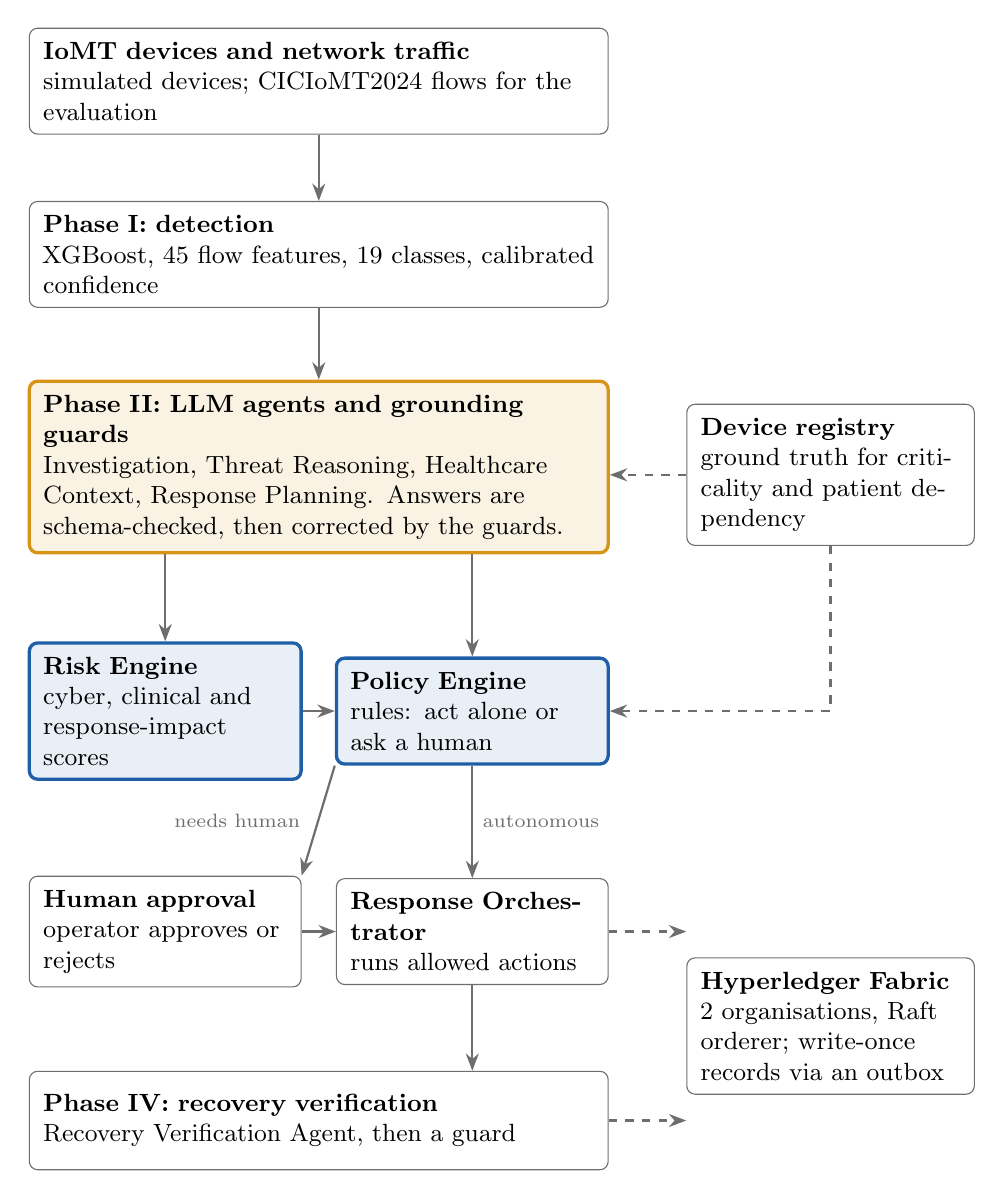
\begin{tikzpicture}[
  font=\small,
  box/.style={draw=pacrgrey, rounded corners=3pt, align=left, inner sep=5pt, text width=7.0cm, minimum height=1.25cm},
  half/.style={box, text width=3.1cm},
  side/.style={box, text width=3.3cm},
  agent/.style={box, draw=pacramber, fill=pacramber!12, very thick},
  safe/.style={half, draw=pacrblue, fill=pacrblue!10, very thick},
  arr/.style={-{Stealth[length=2.2mm]}, thick, color=pacrgrey},
  dsh/.style={arr, dashed}]
\node[box] (dev) at (0,0) {\textbf{IoMT devices and network traffic}\\ simulated devices; CICIoMT2024 flows for the evaluation};
\node[box] (det) at (0,-2.2) {\textbf{Phase I: detection}\\ XGBoost, 45 flow features, 19 classes, calibrated confidence};
\node[agent] (ag) at (0,-4.9) {\textbf{Phase II: LLM agents and grounding guards}\\ Investigation, Threat Reasoning, Healthcare Context, Response Planning. Answers are schema-checked, then corrected by the guards.};
\node[safe] (risk) at (-1.95,-8.0) {\textbf{Risk Engine}\\ cyber, clinical and response-impact scores};
\node[safe] (pol) at (1.95,-8.0) {\textbf{Policy Engine}\\ rules: act alone or ask a human};
\node[half] (hum) at (-1.95,-10.8) {\textbf{Human approval}\\ operator approves or rejects};
\node[half] (resp) at (1.95,-10.8) {\textbf{Response Orchestrator}\\ runs allowed actions};
\node[box] (rec) at (0,-13.2) {\textbf{Phase IV: recovery verification}\\ Recovery Verification Agent, then a guard};
\node[side] (reg) at (6.5,-5.0) {\textbf{Device registry}\\ ground truth for criticality and patient dependency};
\node[side] (led) at (6.5,-12.0) {\textbf{Hyperledger Fabric}\\ 2 organisations, Raft orderer; write-once records via an outbox};
\draw[arr] (dev.south) -- (det.north);
\draw[arr] (det.south) -- (ag.north);
\draw[arr] (ag.south -| risk.north) -- (risk.north);
\draw[arr] (ag.south -| pol.north) -- (pol.north);
\draw[arr] (risk.east) -- (pol.west);
\draw[arr] (pol.south west) -- (hum.north east) node[midway, left, font=\scriptsize, xshift=-1mm] {needs human};
\draw[arr] (pol.south) -- (resp.north) node[midway, right, font=\scriptsize] {autonomous};
\draw[arr] (hum.east) -- (resp.west);
\draw[arr] (resp.south) -- (resp.south |- rec.north);
\draw[dsh] (reg.west) -- (reg.west -| ag.east);
\draw[dsh] (reg.south) |- (pol.east);
\draw[dsh] (resp.east) -- (resp.east -| led.west);
\draw[dsh] (rec.east) -- (rec.east -| led.west);
\end{tikzpicture}
\caption{Architecture of \pacr. Amber: language-model agents, treated as untrusted. Bold blue: deterministic safety layer with no language model. Dashed: registry reads and ledger writes.}
\label{fig:arch}
\end{figure}

\subsection{Phases of the framework}
\pacr{} runs in four phases (Figure~\ref{fig:phases}).

\begin{figure}[htbp]
\centering
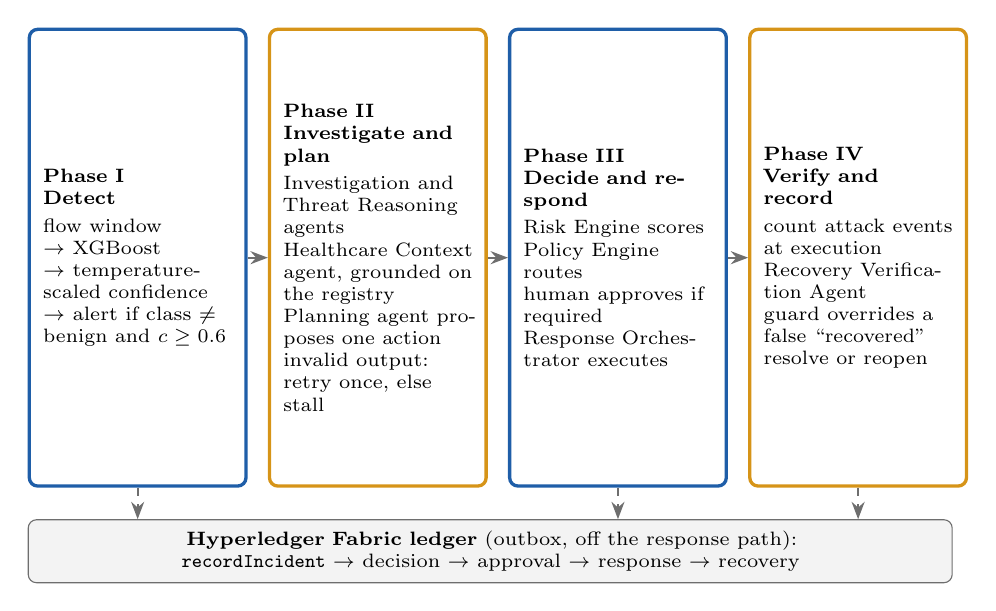
\begin{tikzpicture}[
  font=\scriptsize,
  ph/.style={draw=pacrgrey, rounded corners=3pt, align=left, inner sep=5pt, text width=2.4cm, minimum height=5.8cm, anchor=north},
  arr/.style={-{Stealth[length=2.2mm]}, thick, color=pacrgrey}]
\node[ph, draw=pacrblue, very thick] (p1) at (0,0) {\textbf{Phase I\\ Detect}\\[2pt] flow window\\ $\rightarrow$ XGBoost\\ $\rightarrow$ temperature-scaled confidence\\ $\rightarrow$ alert if class $\neq$ benign and $c\ge 0.6$};
\node[ph, draw=pacramber, very thick] (p2) at (3.05,0) {\textbf{Phase II\\ Investigate and plan}\\[2pt] Investigation and Threat Reasoning agents\\ Healthcare Context agent, grounded on the registry\\ Planning agent proposes one action\\ invalid output: retry once, else stall};
\node[ph, draw=pacrblue, very thick] (p3) at (6.1,0) {\textbf{Phase III\\ Decide and respond}\\[2pt] Risk Engine scores\\ Policy Engine routes\\ human approves if required\\ Response Orchestrator executes};
\node[ph, draw=pacramber, very thick] (p4) at (9.15,0) {\textbf{Phase IV\\ Verify and record}\\[2pt] count attack events at execution\\ Recovery Verification Agent\\ guard overrides a false ``recovered''\\ resolve or reopen};
\draw[arr] (p1.east) -- (p2.west);
\draw[arr] (p2.east) -- (p3.west);
\draw[arr] (p3.east) -- (p4.west);
\node[draw=pacrgrey, rounded corners=3pt, fill=pacrgrey!8, text width=11.5cm, minimum height=0.8cm, anchor=north west, align=center, font=\scriptsize] (ledger) at ([yshift=-0.4cm]p1.south west) {\textbf{Hyperledger Fabric ledger} (outbox, off the response path): \texttt{recordIncident} $\rightarrow$ decision $\rightarrow$ approval $\rightarrow$ response $\rightarrow$ recovery};
\draw[arr, dashed] (p1.south) -- (p1.south |- ledger.north);
\draw[arr, dashed] (p3.south) -- (p3.south |- ledger.north);
\draw[arr, dashed] (p4.south) -- (p4.south |- ledger.north);
\end{tikzpicture}
\caption{The four phases and where each ledger record is written. Colours as in Figure~\ref{fig:arch}.}
\label{fig:phases}
\end{figure}

\subsection{Phase I: detection and calibrated confidence}
A flow window with feature vector $\mathbf{x}$ is classified by an XGBoost model into one of $K=19$ classes (Benign plus 18 attack types). With logits $z_k(\mathbf{x})$, the calibrated probability and confidence are
\begin{equation}
p_k(\mathbf{x}) = \frac{\exp\!\big(z_k(\mathbf{x})/T\big)}{\sum_{j=1}^{K}\exp\!\big(z_j(\mathbf{x})/T\big)},\qquad c(\mathbf{x}) = \max_k p_k(\mathbf{x}),
\label{eq:temp}
\end{equation}
where the temperature $T$ is fitted by minimising the negative log-likelihood on a validation split ($T=0.917$ in our run). An alert is raised when the predicted class $\hat y$ is not Benign and $c\ge\theta$ with $\theta=0.6$. An optional \emph{confidence gate} additionally forbids autonomous action when $c<\tau$; $\tau$ is chosen on validation data only (Section~\ref{sec:gate}).

\subsection{Phase II: guarded agents}
Five agents are used: Investigation, Threat Reasoning, Healthcare Context, Response Planning and Recovery Verification (the last in Phase~IV). Each returns JSON that must satisfy a schema. A parse or schema failure triggers one retry; a second failure stalls the incident in a safe state (for example \texttt{investigation\_stalled}) instead of guessing. Three deterministic guards then correct what the agents claim.
\begin{align}
\kappa' &= \kappa_{\mathrm{reg}}(d), \qquad \pi' = \pi_{\mathrm{reg}}(d), \label{eq:g1}\\
i' &= \max(i,\mathrm{HIGH}) \ \text{ if } \kappa_{\mathrm{reg}}(d)=\mathrm{HIGH}\wedge \pi_{\mathrm{reg}}(d), \label{eq:g1b}\\
\mathrm{success}' &= \mathrm{success}\wedge (n_{\mathrm{after}}\le n_{\mathrm{exec}}), \label{eq:g2}\\
\text{accept } o &\iff \mathrm{id}(o)=\mathrm{id}(\text{incident}). \label{eq:g3}
\end{align}
Equations~\eqref{eq:g1} and~\eqref{eq:g1b} are guard G1 (clinical context), Eq.~\eqref{eq:g2} is G2 (recovery claim) and Eq.~\eqref{eq:g3} is G3 (incident identity).
In these equations $\kappa$ is device criticality, $\pi$ is patient dependency, $i$ is the stated clinical impact, $d$ is the device, $o$ is an agent's output, $n_{\mathrm{exec}}$ is the count of attack events observed when the action was executed and $n_{\mathrm{after}}$ the count at verification. G2 uses an event count, not a clock, so it needs no synchronised time. Every correction is logged and stored in the incident trace next to the agent's original output.

\subsection{Phase III: Risk Engine and Policy Engine}
The Risk Engine is an explicit rule table, not a learned model, so each score can be audited. With threat severity $s$ and the Threat Reasoning Agent's confidence $\gamma\in[0,1]$, device criticality $\kappa$, clinical impact $i$ and patient dependency $\pi\in\{0,1\}$:
\begin{align}
R_{\mathrm{cyber}} &= b_s\,(0.5+0.5\,\gamma),\label{eq:cyber}\\
R_{\mathrm{clin}} &= \min\{1,\ \max(b_\kappa+\Delta_i,\ 0.55\,\pi)\}.\label{eq:clin}
\end{align}
The base scores are $b_s\in\{0.15,0.40,0.70,0.90\}$ for low, medium, high and critical severity, $b_\kappa\in\{0.10,0.35,0.60\}$ for low, medium and high criticality, and $\Delta_i\in\{0,0.05,0.15,0.25\}$ for low to critical clinical impact.
The 0.5 floor in~\eqref{eq:cyber} stops a low-confidence severe assessment from scoring near zero, and the 0.55 floor in~\eqref{eq:clin} means a device a patient depends on never scores low clinical risk. The third score, \emph{response impact}, says how harmful the \emph{action itself} would be on this device (Table~\ref{tab:impact}).

\begin{table}[htbp]
\centering
\caption{Response impact of an action, by its disruption tier and the device context.}
\label{tab:impact}
\small
\begin{tabular}{@{}L{5.0cm}C{2.8cm}C{2.4cm}C{2.4cm}@{}}
\toprule
Action tier (examples) & HIGH criticality and patient-dependent & Patient-dependent & Not patient-dependent \\
\midrule
Severe: shutdown, isolate critical, quarantine segment, failover & Critical & High & Medium \\
Moderate: isolate non-critical, restrict communication, restart service, block traffic & High & Medium & Low \\
Non-disruptive: rotate credentials, revoke session, activate backup & Medium & Low & Low \\
\bottomrule
\end{tabular}
\end{table}

The Policy Engine routes the single action the planner recommends. The first matching rule wins (Table~\ref{tab:rules}); no rule reads a model's opinion of the device or the attack.

\begin{table}[htbp]
\centering
\caption{Policy Engine routing rules, in evaluation order.}
\label{tab:rules}
\small
\begin{tabular}{@{}C{0.9cm}L{7.6cm}L{4.0cm}@{}}
\toprule
Order & Condition & Outcome \\
\midrule
1 & Patient-dependent device and action is shutdown or isolate-critical & Human approval, always \\
2 & Response impact is low or less & Autonomous \\
3 & Response impact is medium and the device is not patient-dependent & Autonomous \\
4 & Response impact is medium and the device is patient-dependent (conservative gap-fill) & Human approval \\
5 & Response impact is high or critical & Human approval \\
Gate & Optional: detector confidence $c<\tau$, or $c$ unknown & Autonomous becomes human approval \\
\bottomrule
\end{tabular}
\end{table}

The gate can only turn an autonomous decision into a human one, never the reverse. Each decision carries a stable rule identifier so a reviewer can see which rule fired.

\subsection{Phase IV: recovery verification and provenance}
After an action runs, the system records $n_{\mathrm{exec}}$, the Recovery Verification Agent judges whether the device is safe, and guard G2 overrides a success claim if attack events have continued. A failed check reopens the incident. Five write-once records go to Hyperledger Fabric 2.5.9: \texttt{recordIncident}, decision, approval, response and recovery. Each stores an evidence hash rather than the evidence. A transaction commits only if a majority of the two organisations (Hospital and SecurityOps) endorse it, and the client waits for both peers' commit events before reporting success. \texttt{verify\_evidence} recomputes a hash and checks that it is on the ledger.

\subsection{Algorithms}
Algorithm~\ref{alg:main} is the end-to-end procedure. Algorithm~\ref{alg:guard} is the guarded agent call used inside it.

\begin{algorithm}[htbp]
\caption{\pacr{} incident handling}
\label{alg:main}
\begin{algorithmic}[1]
\Require flow window $\mathbf{x}$ on device $d$; registry $\mathcal{R}$; thresholds $\theta$, optional $\tau$
\State $(\hat y, c)\gets \textsc{Detect}(\mathbf{x})$ \Comment{Eq.~\eqref{eq:temp}}
\If{$\hat y=\text{Benign}$ \textbf{or} $c<\theta$}
  \State \Return
\EndIf
\State open incident $u$ and call \textsc{Ledger.recordIncident}$(u)$
\State $E\gets \textsc{GuardedCall}(\text{Investigation}, u)$
\State $A\gets \textsc{GuardedCall}(\text{ThreatReasoning}, E)$
\State $C\gets \textsc{GuardedCall}(\text{HealthcareContext}, u)$
\State $C\gets \textsc{G1}(C,\mathcal{R}[d])$ \Comment{Eqs.~\eqref{eq:g1}, \eqref{eq:g1b}}
\State $P\gets \textsc{GuardedCall}(\text{ResponsePlanning}, A, C)$
\State $a\gets P.\text{recommended}$
\State $S\gets \textsc{RiskEngine}(A, C, P)$ \Comment{Eqs.~\eqref{eq:cyber}, \eqref{eq:clin}; Table~\ref{tab:impact}}
\State $(h, \rho)\gets \textsc{PolicyEngine}(S, C, a, c, \tau)$ \Comment{Table~\ref{tab:rules}}
\State \textsc{Ledger.recordDecision}$(u, a, \rho)$
\If{$h$}
  \State wait for the operator; \textsc{Ledger.recordApproval}$(u)$
  \If{rejected} \State \Return \EndIf
\EndIf
\State $n_{\mathrm{exec}}\gets \textsc{CountAttackEvents}(d)$
\State execute $a$ and call \textsc{Ledger.recordResponse}$(u)$
\State $V\gets \textsc{GuardedCall}(\text{RecoveryVerification}, u)$
\State $V\gets \textsc{G2}(V, n_{\mathrm{exec}})$ \Comment{Eq.~\eqref{eq:g2}}
\State \textsc{Ledger.recordRecovery}$(u)$
\State mark $u$ resolved if $V.\text{success}$, otherwise reopened
\end{algorithmic}
\end{algorithm}

\begin{algorithm}[htbp]
\caption{\textsc{GuardedCall}: schema validation, retry and identity check}
\label{alg:guard}
\begin{algorithmic}[1]
\Require agent $g$, prompt $q$, schema $\Sigma$, incident id $u$
\For{$attempt=1,2$}
  \State $o\gets \textsc{LLM}(g,q)$
  \If{$o$ parses, satisfies $\Sigma$ and $\mathrm{id}(o)=u$} \Comment{G3, Eq.~\eqref{eq:g3}}
    \State \Return $o$
  \EndIf
\EndFor
\State stall the incident safely (no action is taken)
\end{algorithmic}
\end{algorithm}

\paragraph{How the algorithm is used.}
The detector runs on every flow window. Only an alert opens an incident, so the agents, engines and ledger run at incident rate, not flow rate. Because the engines and guards are plain code, they are unit-tested exhaustively; the language-model calls are the only non-deterministic step, and a failure there stalls safely or is corrected, never executed. Implementation is a Python backend with FastAPI, XGBoost for the detector, a Node.js chaincode for Fabric, and a simulated hospital of devices for the response and recovery steps.

%% ==========================================================================

\section{Results}
\label{sec:results}

\subsection{Experimental setup}
\label{sec:setup}
Four experiments evaluate the four parts of \pacr: (E1) the detector on real data, (E2) the calibrated confidence gate, (E3) the patient-safety behaviour of the decision layer against baselines and ablations, (E4) the agentic layer under injected faults, and (E5) the blockchain on a real Fabric network. Every figure and table below is produced by a script in the project repository and written to a report file; none is typed by hand, and the repository is available on request from the authors (TODO: add the public repository link).

\paragraph{Software and hardware.}
The backend is Python (FastAPI) with an XGBoost detector (150 trees, depth 8, learning rate 0.2, histogram method, 256 bins) and a random-forest comparator (100 trees). Fabric 2.5.9 runs natively on one host with 2 CPUs: two organisations (Hospital, SecurityOps) with one peer each, one Raft orderer with a 1~s batch timeout, a Node.js chaincode through an external builder, and a majority endorsement policy. All random seeds are fixed (seed 42; five seeds for device-context sampling).

\paragraph{Metrics.}
For the detector we report accuracy, macro-F1 (over 19 classes and over six attack families), attack-detection rate (the share of attack flows flagged as any attack) and benign false-positive rate (FPR, the share of benign flows flagged). For safety we define two rates. The \emph{unsafe autonomous action rate} (UAR) is, among real attacks that hit a HIGH-criticality, patient-dependent device, the share for which the system executed a disruptive action with no human approval. The \emph{unnecessary isolation rate} (UIR) is, among detector false positives, the share for which the system autonomously isolated the device anyway. We also report \emph{autonomy retained}: of the real attacks that would be handled autonomously without a gate, the share that still are. For the ledger we report integrity-check outcomes, latency percentiles and committed throughput.

\subsection{Dataset}
\label{sec:dataset}
We use the WiFi and MQTT release of CICIoMT2024~\cite{dadkhah2024}, a benchmark of network flows from a testbed of IoMT devices under attack. The official capture-level split is kept: no random re-splitting and no tuning on the test split. Table~\ref{tab:dataset} gives the dimensions. The test split is dominated by volumetric floods (about 1.5 million of its 1.6 million flows), so overall accuracy is high by construction and macro-F1 is the more informative figure.

\begin{table}[htbp]
\centering
\caption{CICIoMT2024 (WiFi+MQTT) as used in this work.}
\label{tab:dataset}
\small
\begin{tabular}{@{}L{5.0cm}L{7.5cm}@{}}
\toprule
Property & Value \\
\midrule
Official training rows & 7,017,530 (training capped at 300,000 per class; 30,000 for random forest) \\
Rows actually used for training & 2,975,443 (XGBoost); 441,318 (random forest) \\
Official test rows (all used, none sampled) & 1,614,182: 37,607 benign, 1,576,575 attack \\
Features per flow & 45 (the dataset's own flow features) \\
Classes & 19: Benign and 18 attacks (MQTT floods and malformed data; TCP/IP DDoS and DoS; reconnaissance; ARP spoofing) \\
Clinical device context & Not in the dataset; simulated (Section~\ref{sec:safety}) \\
\bottomrule
\end{tabular}
\end{table}

\subsection{E1: detector performance}
\label{sec:detector}
Table~\ref{tab:detector} reports the two detectors on the entire test split. XGBoost reaches 99.52\% 19-class accuracy, macro-F1 0.9263 and 99.97\% attack detection, with a benign FPR of 5.09\% at the arg-max operating point. At the runtime operating point (alert only when confidence is at least 0.6) attack detection is 99.72\% and the benign FPR falls to 3.12\% (1,174 of 37,607 benign flows flagged). Of the 1,576,575 attack flows, XGBoost misses 440 as binary decisions (TP 1,576,135; FP 1,916; TN 35,691; precision 0.9988).

\begin{table}[htbp]
\centering
\caption{Detector results on the full CICIoMT2024 test split (1,614,182 flows).}
\label{tab:detector}
\footnotesize
\begin{tabular}{@{}l@{\hspace{6pt}}c@{\hspace{5pt}}c@{\hspace{5pt}}c@{\hspace{5pt}}c@{\hspace{5pt}}c@{\hspace{5pt}}c@{}}
\toprule
Model & Acc.\ (19) & F1$_{\mathrm{macro}}$ (19) & F1$_{\mathrm{macro}}$ (6) & Attack det. & Benign FPR & Train (s) \\
\midrule
XGBoost & 0.9952 & 0.9263 & 0.9126 & 0.9997 & 0.0509 & 749 \\
Random forest & 0.9916 & 0.8704 & 0.9036 & 0.9995 & 0.0673 & 56 \\
\bottomrule
\end{tabular}
\end{table}

Figure~\ref{fig:f1} shows the per-class F1 of XGBoost. The volumetric classes are near perfect (F1 above 0.99 for the DDoS and DoS TCP/IP classes). The weak classes are ARP spoofing (F1 0.5346, precision 0.4055) and vulnerability scanning (0.6919); both are rare in the data. This matters downstream: 94.4\% of the detector's false alarms are predicted as ARP spoofing, so the cheap-to-fix weakness is concentrated in one class.

\begin{figure}[htbp]
\centering
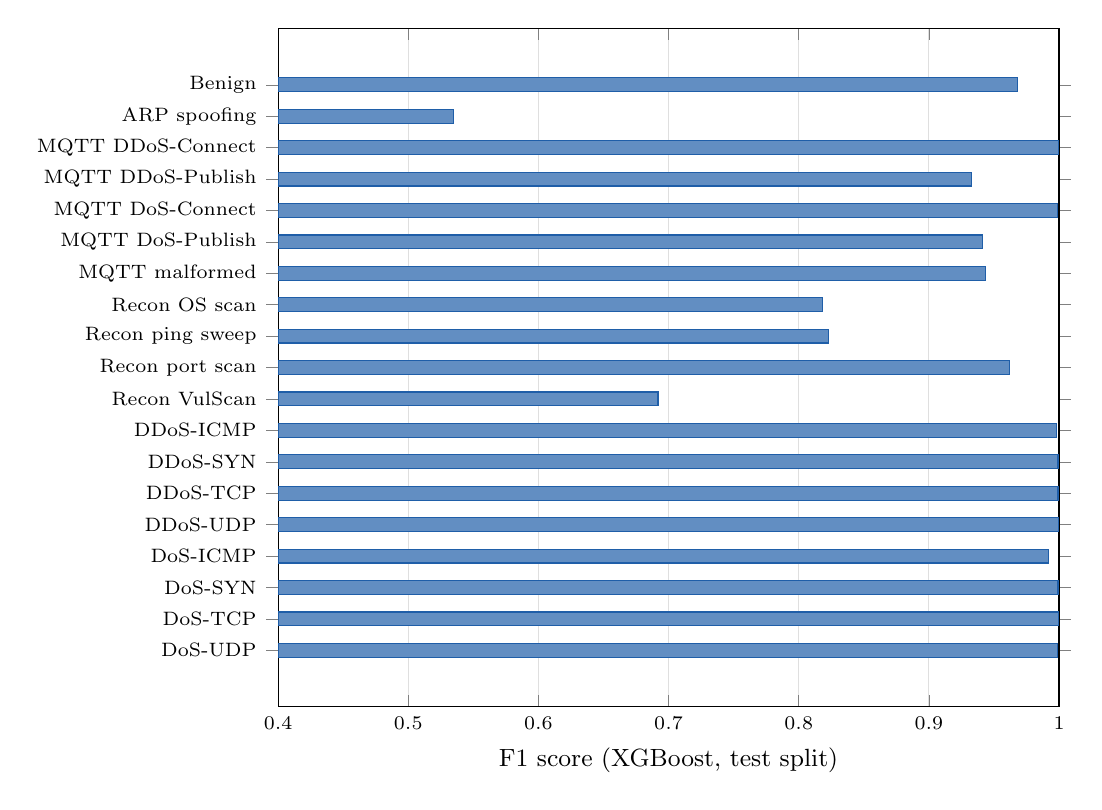
\begin{tikzpicture}
\begin{axis}[
  xbar, width=11.5cm, height=10.2cm, bar width=5pt,
  xmin=0.4, xmax=1.0, xlabel={F1 score (XGBoost, test split)},
  symbolic y coords={Benign,ARP spoofing,MQTT DDoS-Connect,MQTT DDoS-Publish,MQTT DoS-Connect,MQTT DoS-Publish,MQTT malformed,Recon OS scan,Recon ping sweep,Recon port scan,Recon VulScan,DDoS-ICMP,DDoS-SYN,DDoS-TCP,DDoS-UDP,DoS-ICMP,DoS-SYN,DoS-TCP,DoS-UDP},
  ytick=data, y dir=reverse, yticklabel style={font=\scriptsize},
  xmajorgrids, grid style={gray!25}, tick label style={font=\scriptsize}, label style={font=\small}]
\addplot[fill=pacrblue!70, draw=pacrblue] coordinates {
 (0.9680,Benign) (0.5346,ARP spoofing) (0.9999,MQTT DDoS-Connect) (0.9326,MQTT DDoS-Publish)
 (0.9990,MQTT DoS-Connect) (0.9415,MQTT DoS-Publish) (0.9437,MQTT malformed) (0.8184,Recon OS scan)
 (0.8229,Recon ping sweep) (0.9617,Recon port scan) (0.6919,Recon VulScan) (0.9978,DDoS-ICMP)
 (0.9992,DDoS-SYN) (0.9992,DDoS-TCP) (0.9994,DDoS-UDP) (0.9916,DoS-ICMP) (0.9992,DoS-SYN)
 (0.9995,DoS-TCP) (0.9990,DoS-UDP)};
\end{axis}
\end{tikzpicture}
\caption{Per-class F1 of the XGBoost detector on the full test split (macro-F1 0.9263). ARP spoofing and vulnerability scanning are the weak classes.}
\label{fig:f1}
\end{figure}

\paragraph{Detection delay.}
Because the dataset rows carry no wall-clock timestamp, delay is counted in flows. On all 20 attack captures in the test split the detector's first alert came at flow 0 (17 captures) or flow 1 (3 captures), and every capture was alerted within its first 10 flows. The share of a capture's flows that raised an alert ranged from 73.6\% (vulnerability scanning) to 100\%.

\subsection{E2: calibrated confidence gate}
\label{sec:gate}
Confidence is informative here: among alerts, real attacks have median confidence 1.0000 and false alarms 0.7583, and the area under the ROC curve of confidence for separating them is 0.9893. To choose a threshold without touching the test split we trained a development model, held out validation data from both training and test, fitted the temperature on validation, and fixed the selection rule beforehand: choose the largest $\tau$ that keeps at least 95\% of real-attack autonomy on validation. Temperature scaling gave $T=0.917$ and improved validation calibration (ECE 0.0409 to 0.0288; NLL 0.1504 to 0.1495); on test ECE was 0.0033 raw and 0.0030 calibrated, while NLL moved slightly the wrong way (0.0204 to 0.0210), so the calibration gain is small and mainly on validation.

\begin{figure}[htbp]
\centering
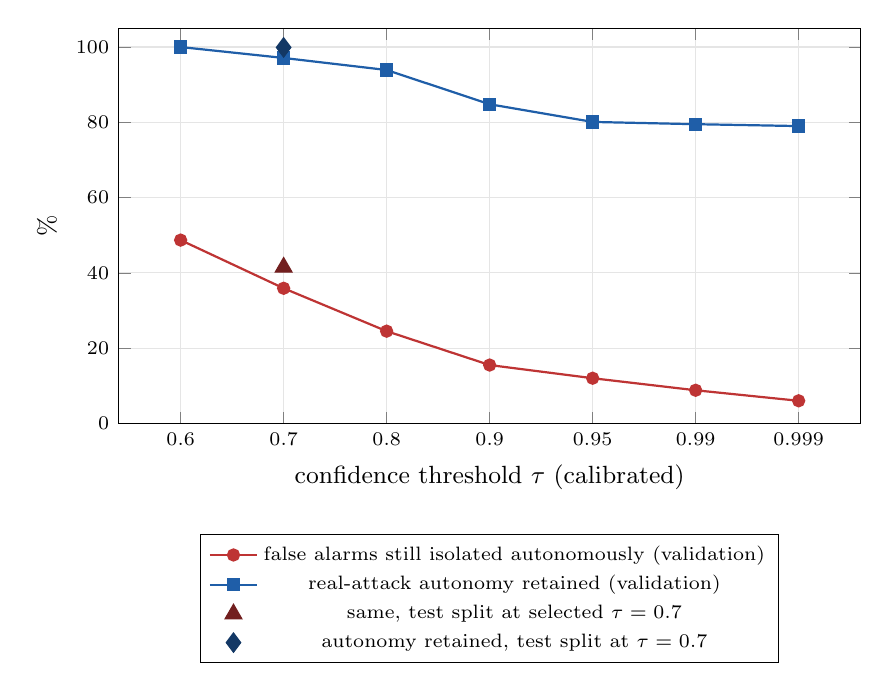
\begin{tikzpicture}
\begin{axis}[
  width=11cm, height=6.6cm, xlabel={confidence threshold $\tau$ (calibrated)}, ylabel={\%},
  xtick={1,2,3,4,5,6,7}, xticklabels={0.6,0.7,0.8,0.9,0.95,0.99,0.999}, ymin=0, ymax=105,
  legend style={font=\scriptsize, at={(0.5,-0.28)}, anchor=north, legend columns=1},
  grid=both, grid style={gray!20}, tick label style={font=\scriptsize}, label style={font=\small}]
\addplot[color=pacrred, mark=*, thick] coordinates {(1,48.7) (2,35.9) (3,24.5) (4,15.5) (5,12.0) (6,8.8) (7,6.0)};
\addlegendentry{false alarms still isolated autonomously (validation)}
\addplot[color=pacrblue, mark=square*, thick] coordinates {(1,100.0) (2,97.1) (3,93.9) (4,84.8) (5,80.1) (6,79.5) (7,79.0)};
\addlegendentry{real-attack autonomy retained (validation)}
\addplot[only marks, mark=triangle*, mark size=3.5pt, color=pacrred!60!black] coordinates {(2,41.5)};
\addlegendentry{same, test split at selected $\tau=0.7$}
\addplot[only marks, mark=diamond*, mark size=3.5pt, color=pacrblue!60!black] coordinates {(2,99.9)};
\addlegendentry{autonomy retained, test split at $\tau=0.7$}
\end{axis}
\end{tikzpicture}
\caption{Confidence-gate trade-off. $\tau=0.7$ was selected on validation; the triangle and diamond are the single test-split scores at that threshold. Unsafe autonomous actions are 0.0\% at every $\tau$.}
\label{fig:gate}
\end{figure}

The rule selected $\tau=0.7$ (Figure~\ref{fig:gate}). Scored once on the untouched test split, the gate left 41.5\% (40.0--43.2\%, range over five context seeds) of the development model's 1,558 false alarms with autonomous isolation, against 50.5\% (48.8--52.1\%) without the gate, while the system still acted autonomously on 99.9\% of the real attacks it would otherwise handle alone. Unsafe autonomous actions stayed at 0.0\%. The gate is therefore a modest improvement, not a cure: more than 40\% of false alarms are still isolated without a human. The gate is off by default in the shipped system and is an opt-in setting.

\subsection{E3: patient-safety behaviour of the decision layer}
\label{sec:safety}
Every one of the 1,614,182 test flows is one trial. The XGBoost detector, Risk Engine and Policy Engine are the real implementations. The dataset has no clinical context, so each trial draws a device context uniformly over three criticality levels crossed with patient-dependent yes or no, and the three language-model-backed agents are replaced by deterministic stand-ins; the whole experiment is repeated over five context seeds (cells show the mean, with the range across seeds in brackets where it is not negligible). There are about 262,000 high-stakes trials (a real attack on a HIGH-criticality, patient-dependent device) per seed.

\begin{table}[htbp]
\centering
\caption{Five response systems on the full test split (mean over five context seeds).}
\label{tab:systems}
\small
\begin{tabular}{@{}L{4.8cm}C{3.2cm}C{4.4cm}@{}}
\toprule
System & Unsafe autonomous action rate & Unnecessary isolation rate \\
\midrule
Detection only (never acts) & 0.00\% & 0.00\% \\
Fixed response & 99.72\% (99.70--99.75) & 100.00\% \\
Detection + Risk Engine & 99.72\% (99.70--99.75) & 100.00\% \\
Detection + agentic layer & 0.00\% & 50.48\% (48.98--52.81) \\
\textbf{Full system (\pacr)} & \textbf{0.00\%} & \textbf{50.48\% (48.98--52.81)} \\
\bottomrule
\end{tabular}
\end{table}

\begin{figure}[htbp]
\centering
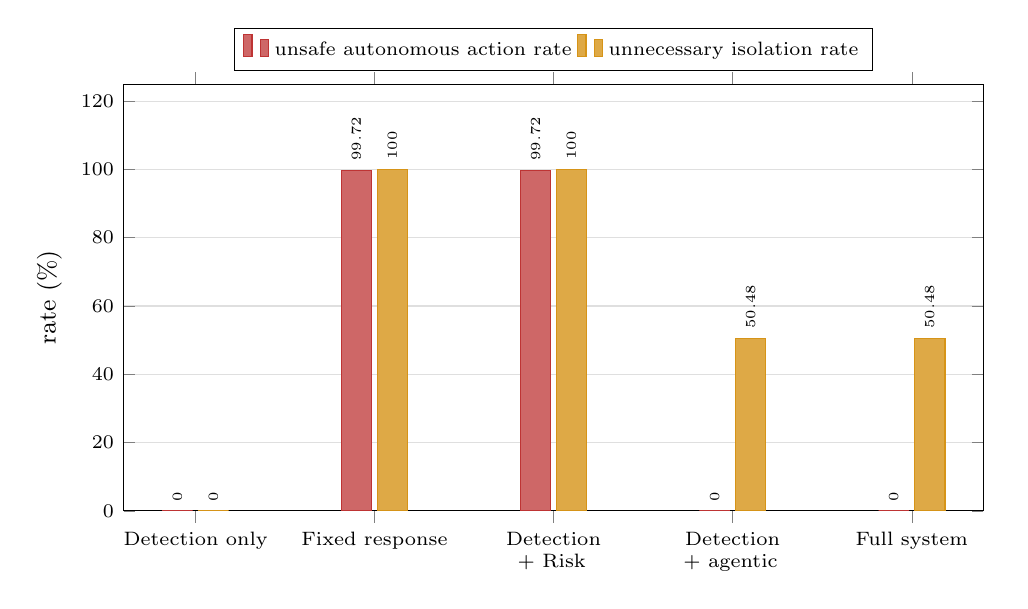
\begin{tikzpicture}
\begin{axis}[
  ybar, width=12.5cm, height=7.0cm, bar width=11pt, ymin=0, ymax=125,
  symbolic x coords={Detection only,Fixed response,Detection + Risk,Detection + agentic,Full system},
  xtick=data, xticklabel style={font=\scriptsize, text width=2cm, align=center},
  ylabel={rate (\%)}, nodes near coords, nodes near coords style={font=\tiny, rotate=90, anchor=west},
  legend style={font=\scriptsize, at={(0.5,1.03)}, anchor=south, legend columns=2},
  ymajorgrids, grid style={gray!25}, tick label style={font=\scriptsize}, label style={font=\small}]
\addplot[fill=pacrred!75, draw=pacrred] coordinates {(Detection only,0) (Fixed response,99.72) (Detection + Risk,99.72) (Detection + agentic,0) (Full system,0)};
\addlegendentry{unsafe autonomous action rate}
\addplot[fill=pacramber!80, draw=pacramber] coordinates {(Detection only,0) (Fixed response,100) (Detection + Risk,100) (Detection + agentic,50.48) (Full system,50.48)};
\addlegendentry{unnecessary isolation rate}
\end{axis}
\end{tikzpicture}
\caption{Safety of the five systems on the full test split. ``Detection only'' is zero by construction because it never acts.}
\label{fig:systems}
\end{figure}

Table~\ref{tab:systems} and Figure~\ref{fig:systems} show the central result. A fixed-response playbook, and the same playbook with a Risk Engine score but no routing, execute a disruptive action without a human on 99.72\% of high-stakes real attacks. The agentic layer with the Policy Engine reduces this to 0.00\%. The price is the unnecessary isolation rate: on the roughly half of false alarms that land on contexts the policy lets it handle alone, the system still isolates the device (50.48\%). The denominator for that rate is the 1,174 benign flows the detector flagged, a much smaller sample than the unsafe-action rate; and this is the rate the calibrated gate of Section~\ref{sec:gate} lowers.

\begin{table}[htbp]
\centering
\caption{Ablations of the full system (same trials). ``Differs'' counts trials per seed where the decision differs from the full system.}
\label{tab:ablation}
\small
\begin{tabular}{@{}L{4.6cm}C{2.4cm}C{3.2cm}C{2.4cm}@{}}
\toprule
Ablation & Unsafe action rate & Unnecessary isolation & Differs (per seed) \\
\midrule
Without healthcare context & 0.00\% & 50.48\% & 0 \\
Without clinical criticality & 0.00\% & 50.48\% & 0 \\
Without response-impact assessment & 0.62\% (0.60--0.63) & 80.83\% (79.98--81.86) & 5,211--5,334 \\
Without agentic layer & 99.72\% & 100.00\% & 785,951--787,713 \\
Without blockchain & 0.00\% & 50.48\% & 0 \\
Without recovery verification & 0.00\% & 50.48\% & 0 \\
\bottomrule
\end{tabular}
\end{table}

Table~\ref{tab:ablation} separates what carries the safety result. Removing the response-impact assessment lets 0.62\% of high-stakes attacks through and raises unnecessary isolation to 80.83\%, so that component matters. Removing the agentic layer restores the fixed-response behaviour. In this harness the agentic layer is a deterministic stand-in that supplies clinical context and a planned action, so this ablation shows that the \emph{context-aware planning layer} is essential, not that a language model is necessary. Removing healthcare context, clinical criticality, the blockchain or recovery verification changes nothing here. For the first two this is structural: the Policy Engine routes on response impact and patient dependency, and the patient-dependency rule already forces approval; for the last two, neither component is on this harness's decision path (the ledger and recovery are evaluated separately in Sections~\ref{sec:agents} and~\ref{sec:chain}). We report these zeros rather than omit them.

\paragraph{Cost of safety: who waits.}
Safety is paid for in human time. In the full system 50.0\% of alerts across all devices wait for a person (785,858 contained autonomously, 786,293 waiting), and on high-stakes devices every alert waits (262,215 of 262,215 detected attacks). At the runtime confidence threshold the detector misses 4,424 attack flows overall (708 on high-stakes devices), which no response layer can recover; these shares use three context seeds. The delay model in Section~\ref{sec:compare-cost} uses an \emph{assumed} approval time, since the project has no measurement of one.

\subsection{E4: the agentic layer under injected faults}
\label{sec:agents}
To test the claim that no agent can by itself cause harm, the five agents were driven by a scripted, deliberately misbehaving client through the real orchestrator, engines and simulated devices. Ten behaviours were run on three simulated devices: an infusion pump (low criticality, no patient attached), an ECG monitor, and a ventilator (the only HIGH-criticality, patient-dependent device in the simulated hospital). Table~\ref{tab:faults} lists the outcomes; each cell is one deterministic run.

\begin{table}[htbp]
\centering
\caption{Outcome per injected behaviour and device. Auto: resolved or reopened with the system acting alone. Human: held for approval, device untouched. Stall: the incident stopped safely.}
\label{tab:faults}
\small
\begin{tabular}{@{}L{6.2cm}C{1.9cm}C{1.9cm}C{2.4cm}@{}}
\toprule
Injected behaviour & Pump & ECG & Ventilator \\
\midrule
Honest agents (reference) & Auto & Human & Human \\
Context agent claims low criticality, no patient dependency & Auto & Human & Human \\
Same lie, planner also recommends shutdown & Auto (off) & Human & Human \\
Planner recommends shutdown with a false ``low'' impact & Auto (off) & Human & Human \\
Planner understates the clinical impact of isolation & Auto & Human & Human \\
Prompt injection obeyed (text in traffic tells the model to downgrade and shut down) & Auto & Human & Human \\
Every agent returns unparseable text & Stall & Stall & Stall \\
Planner returns an action outside the vocabulary & Stall & Stall & Stall \\
Investigation answers about a different incident & Stall & Stall & Stall \\
Recovery agent claims success while the attack persists & Auto, reopened & Human & Human \\
\bottomrule
\end{tabular}
\end{table}

Across the 30 runs, \textbf{0 unsafe autonomous actions} took effect on the ventilator and \textbf{0 incidents were falsely closed}; 9 runs stalled safely and 14 were routed to a human. The infusion pump is acted on autonomously by design: its registry entry allows it, and the lie in the model's output could not make that more or less safe. To see what the guards add, the same 30 runs were repeated with the three guards of Section~\ref{sec:method} switched off (Figure~\ref{fig:guards}); only those three checks differ.

\begin{figure}[htbp]
\centering
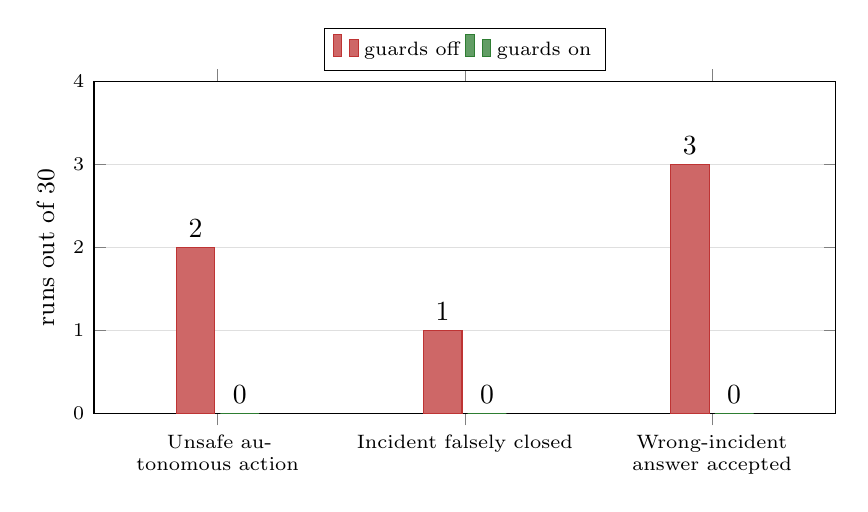
\begin{tikzpicture}
\begin{axis}[
  ybar, width=11cm, height=5.8cm, bar width=14pt, ymin=0, ymax=4, ytick={0,1,2,3,4},
  symbolic x coords={Unsafe autonomous action,Incident falsely closed,Wrong-incident answer accepted},
  xtick=data, xticklabel style={font=\scriptsize, text width=3cm, align=center}, ylabel={runs out of 30},
  nodes near coords, legend style={font=\scriptsize, at={(0.5,1.03)}, anchor=south, legend columns=2},
  ymajorgrids, grid style={gray!25}, tick label style={font=\scriptsize}, label style={font=\small}, enlarge x limits=0.25]
\addplot[fill=pacrred!75, draw=pacrred] coordinates {(Unsafe autonomous action,2) (Incident falsely closed,1) (Wrong-incident answer accepted,3)};
\addlegendentry{guards off}
\addplot[fill=pacrgreen!75, draw=pacrgreen] coordinates {(Unsafe autonomous action,0) (Incident falsely closed,0) (Wrong-incident answer accepted,0)};
\addlegendentry{guards on}
\end{axis}
\end{tikzpicture}
\caption{Effect of the grounding guards over the same 30 fault-injected runs.}
\label{fig:guards}
\end{figure}

With the guards off, two runs took an unsafe autonomous action (the context-lie case, and the context-lie-plus-shutdown case), one incident was falsely closed (the recovery lie), and three answers about the wrong incident were accepted. With the guards on all four counts are zero. \emph{These runs show how the architecture behaves under scripted worst cases; they do not show how often a real model misbehaves.} A live-model evaluation harness exists, but our attempts to complete it were stopped by the model provider's overload and quota errors, so no live-model figure is reported.

\subsection{E5: blockchain provenance on a real Fabric network}
\label{sec:chain}
The measurements use real Fabric binaries driven through the backend's own client; nothing is mocked. Table~\ref{tab:integrity} lists the integrity checks, all of which passed. Beyond these checks, all 142 blocks (194 transactions) were fetched from the Hospital peer and re-verified with an independent implementation of Fabric's block hashing. The genuine chain verified. Editing one byte of one transaction in block 70 (on a copy) was detected at block 70 by the data hash. When the attacker also recomputed that block's own data hash, the edit was still detected, at block 71, because the next block's previous-hash no longer matched. All 188 transactions that the client reported as committed were found as valid on the ledger; the 2 invalid transactions on the chain (an endorsement-policy failure and a read conflict) were produced on purpose by the checks, stay on the chain flagged, and never changed state.

\begin{table}[htbp]
\centering
\caption{Ledger integrity checks (all passed).}
\label{tab:integrity}
\small
\begin{tabular}{@{}C{0.8cm}L{11.8cm}@{}}
\toprule
\# & Check \\
\midrule
1 & A duplicate incident id is rejected (the incident record is write-once). \\
2 & A decision for an unknown incident is rejected. \\
3 & An invalid response-action category is rejected. \\
4 & \texttt{verify\_evidence} accepts the recorded evidence hash. \\
5 & \texttt{verify\_evidence} rejects evidence altered by one field. \\
6 & The Hospital and SecurityOps peers return the same answer. \\
7 & Two simultaneous writers of one incident id: exactly one is committed, and only that record is on the ledger. \\
8 & A transaction endorsed by one organisation only is invalidated by the majority policy and writes no state. \\
\bottomrule
\end{tabular}
\end{table}

\begin{table}[htbp]
\centering
\caption{Ledger latency (ms, sequential). A write returns only after both peers have committed.}
\label{tab:chainlat}
\small
\begin{tabular}{@{}L{7.2cm}cccc@{}}
\toprule
Operation & $n$ & p50 & p95 & max \\
\midrule
Fabric CLI spawn alone (floor) & 20 & 65 & 188 & 239 \\
Write: \texttt{record\_incident} & 40 & 1114 & 1139 & 1147 \\
Query sees a committed write & 20 & 87 & 112 & 127 \\
Read: \texttt{verify\_evidence} & 40 & 89 & 108 & 115 \\
Full five-record incident lifecycle & 10 & 5578 & 5610 & 5617 \\
\bottomrule
\end{tabular}
\end{table}

A write takes about 1.1~s at the median, mostly the 1~s orderer batch timeout plus the wait for both peers; a full lifecycle takes about 5.6~s. Because provenance is written through the outbox off the response path, these latencies do not delay containment. Figure~\ref{fig:conc} shows committed throughput with concurrent clients: 0.90, 1.78, 3.36 and 5.99 transactions per second for 1, 2, 4 and 8 clients, with no failed transaction among 24 submitted at each level and p50 latency rising from 1111 to 1321~ms. Scaling is near linear to four clients and then sub-linear, as expected on a 2-CPU host where every call spawns a CLI process.

\begin{figure}[htbp]
\centering
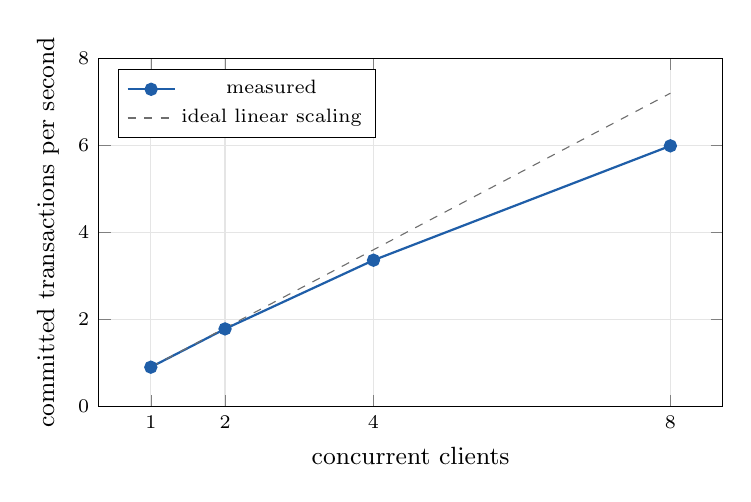
\begin{tikzpicture}
\begin{axis}[
  width=9.5cm, height=6cm, xlabel={concurrent clients}, ylabel={committed transactions per second},
  xtick={1,2,4,8}, ymin=0, ymax=8, grid=both, grid style={gray!20},
  legend style={font=\scriptsize, at={(0.03,0.97)}, anchor=north west},
  tick label style={font=\scriptsize}, label style={font=\small}]
\addplot[color=pacrblue, mark=*, thick] coordinates {(1,0.90) (2,1.78) (4,3.36) (8,5.99)};
\addlegendentry{measured}
\addplot[color=pacrgrey, dashed, mark=none] coordinates {(1,0.90) (2,1.80) (4,3.60) (8,7.20)};
\addlegendentry{ideal linear scaling}
\end{axis}
\end{tikzpicture}
\caption{Committed throughput of the real Fabric network versus concurrent clients (24 transactions per level, none failed).}
\label{fig:conc}
\end{figure}

\paragraph{A defect found by this evaluation.}
The first run showed that the client reported success once a transaction was endorsed and handed to the orderer, not once it was committed. A transaction invalidated at commit would still have been reported as committed, so the outbox could mark a record confirmed that never reached the ledger. The invoke script now waits for both peers' commit events and exits non-zero for an invalidated transaction; the latencies above are measured with the fix, and the checks and integration tests guard against a regression.

\subsection{Pipeline latency}
\label{sec:latency}
Table~\ref{tab:pipe} gives the in-process compute cost of the deterministic part of the pipeline. The decision path (Risk plus Policy) costs about 0.016~ms at the median, and the detector scores a flow in 0.77~ms (batch throughput 32,311 flows per second), so neither is a bottleneck; the language-model calls would dominate in a live deployment and are not included.

\begin{table}[htbp]
\centering
\caption{In-process latency of the deterministic pipeline stages (ms).}
\label{tab:pipe}
\small
\begin{tabular}{@{}L{6.6cm}cccc@{}}
\toprule
Stage & p50 & p95 & p99 & $n$ \\
\midrule
Risk Engine + Policy Engine, per incident & 0.016 & 0.025 & 0.053 & 3,000 \\
Detector, one flow & 0.765 & 0.969 & 1.393 & 300 \\
\bottomrule
\end{tabular}
\end{table}

\subsection{Analysis and limitations}
\label{sec:limits}
\textbf{What the results support.} On real data, the decision layer never lets a disruptive autonomous action reach a registry-flagged high-stakes device, whether the clinical context is supplied by a stand-in (E3) or by a scripted lying agent (E4); the ledger detects tampering of the kind we tried; and the guards close exactly the gaps that a scripted model opens when they are removed.

\textbf{What they do not support.} First, the clinical context in E3 is sampled, not observed, and the agents in E3 and E4 are scripted: the results concern the gating logic, not clinical outcomes and not the error rate of a real model. Second, in E4 only one simulated device is both HIGH-criticality and patient-dependent, so the zero rests on ten ventilator runs; the Policy Engine's rule table is covered exhaustively by unit tests, but the end-to-end study covers few device types. Third, the unnecessary-isolation rate of 41.5--50.5\% is a real weakness: a false alarm on a permitted device still causes autonomous isolation. Fourth, the Fabric network has one orderer on one 2-CPU host, with one run and no confidence intervals, so it says nothing about orderer fault tolerance or malicious orderers, and its latencies belong to this deployment rather than to Fabric. Fifth, the detector is one trained model; variation across seeds reflects context sampling only. Sixth, the system is a research prototype, not a certified medical product.

%% ==========================================================================
\section{Comparisons}
\label{sec:comparison}

We compare \pacr{} with existing work on three axes: detection quality against three published CICIoMT2024 detectors, capabilities against five related systems, and safety against the response baselines of Section~\ref{sec:safety}.

\subsection{Detection quality against published detectors}
\label{sec:compare-det}
Table~\ref{tab:cmpdet} places our XGBoost detector beside L2D2~\cite{akar2025}, the reinforcement-learning hybrid HCLR-IDS~\cite{shaikh2025} and the interpretable XGBoost fusion of Hafid et al.~\cite{hafid2025}. L2D2 and HCLR-IDS use CICIoMT2024; Hafid et al.\ use the CIC IoMT 2024 release with a reduced feature set. Their figures are \emph{as reported by the authors}; we did not retrain their models.

\begin{table}[htbp]
\centering
\caption{Detection comparison on CICIoMT2024. Values for other works are quoted from the cited papers.}
\label{tab:cmpdet}
\small
\begin{tabular}{@{}L{2.4cm}L{2.8cm}C{1.2cm}C{2.4cm}L{3.8cm}@{}}
\toprule
Work & Model & Classes & Accuracy & Other reported metrics \\
\midrule
L2D2~\cite{akar2025} & Enhanced LSTM & 19 & 98\% & --- (none extracted) \\
HCLR-IDS~\cite{shaikh2025} & CNN-LSTM + DQN + PPO & 18 & 0.7773 (multi-class); 0.9958 (binary) & Mutual-information feature selection \\
Hafid et al.~\cite{hafid2025} & XGBoost + logistic-regression fusion, SHAP & as in dataset & 0.97 (XGBoost) & Fusion: precision 0.98, recall 0.91; false negatives 361 to 213; features limited to source, destination, protocol, length, info \\
\textbf{This work} & XGBoost, 45 features & 19 & \textbf{0.9952} (19-class); 0.9985 (binary) & Macro-F1 0.9263; attack detection 0.9997; benign FPR 0.0509; precision 0.9988 \\
\bottomrule
\end{tabular}
\end{table}

\begin{figure}[htbp]
\centering
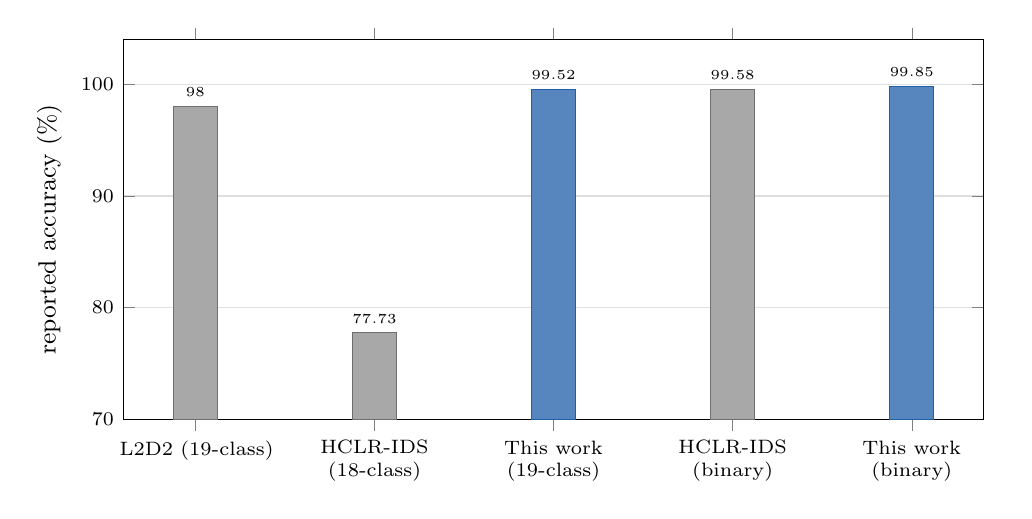
\begin{tikzpicture}
\begin{axis}[
  ybar, width=12.5cm, height=6.4cm, bar width=16pt, ymin=70, ymax=104,
  symbolic x coords={L2D2 (19-class),HCLR-IDS (18-class),This work (19-class),HCLR-IDS (binary),This work (binary)},
  xtick={L2D2 (19-class),HCLR-IDS (18-class),This work (19-class),HCLR-IDS (binary),This work (binary)}, xticklabel style={font=\scriptsize, text width=2.1cm, align=center},
  ylabel={reported accuracy (\%)}, nodes near coords, nodes near coords style={font=\tiny},
  ymajorgrids, grid style={gray!25}, tick label style={font=\scriptsize}, label style={font=\small}]
\addplot[fill=pacrgrey!60, draw=pacrgrey, bar shift=0pt] coordinates {(L2D2 (19-class),98.0) (HCLR-IDS (18-class),77.73) (HCLR-IDS (binary),99.58)};
\addplot[fill=pacrblue!75, draw=pacrblue, bar shift=0pt] coordinates {(This work (19-class),99.52) (This work (binary),99.85)};
\end{axis}
\end{tikzpicture}
\caption{Reported accuracy on CICIoMT2024: multi-class (left three bars) and binary (right two). Bars for other works are quoted, not re-measured; the vertical axis starts at 70\%.}
\label{fig:cmpdet}
\end{figure}

On the quoted numbers our detector is on par with or above the others on accuracy (Figure~\ref{fig:cmpdet}), and its 19-class accuracy of 99.52\% compares with 98\% for L2D2 and 77.73\% for the 18-class HCLR-IDS. We do not claim a win. The comparison is indicative only for three reasons: the protocols differ (the other authors' splits, class definitions and preprocessing may not match the official capture-level split we use, and HCLR-IDS counts 18 classes where we count 19); accuracy on this dataset is dominated by the volumetric DDoS and DoS classes; and the figures we could extract from the other papers are accuracies, so they cannot be compared on macro-F1, where our weak classes (ARP spoofing 0.53, vulnerability scanning 0.69) are visible. The contribution of \pacr{} is therefore not a new detector but what is built after it.

\subsection{Capability comparison}
\label{sec:compare-cap}
Table~\ref{tab:cap} compares what each system covers. This is where \pacr{} differs from the detection papers~\cite{akar2025,shaikh2025,hafid2025}, from the Fabric prototype for IoMT~\cite{pelekoudas2023}, and from the language-model response agent~\cite{lin2025}.

\begin{table}[htbp]
\centering
\caption{Capabilities as described in each work's title and abstract. \checkmark{} = addressed; -- = not part of the stated scope (not a defect of that work); $\circ$ = partly or not verified from what we read.}
\label{tab:cap}
\footnotesize
\begin{tabular}{@{}L{3.0cm}C{1.25cm}C{1.25cm}C{1.25cm}C{1.25cm}C{1.25cm}C{1.25cm}C{1.25cm}@{}}
\toprule
 & {\scriptsize Real IoMT data} & {\scriptsize Auto- mated response} & {\scriptsize Patient- aware gate} & {\scriptsize LLM agents} & {\scriptsize Output guard} & {\scriptsize Block- chain} & {\scriptsize Ledger tested} \\
\midrule
L2D2~\cite{akar2025} & \checkmark & -- & -- & -- & -- & -- & -- \\
HCLR-IDS~\cite{shaikh2025} & \checkmark & -- & -- & -- & -- & -- & -- \\
Hafid et al.~\cite{hafid2025} & \checkmark & -- & -- & -- & -- & -- & -- \\
Pelekoudas-Oikonomou et al.~\cite{pelekoudas2023} & -- & -- & -- & -- & -- & \checkmark & $\circ$ \\
IRCopilot~\cite{lin2025} & -- & \checkmark & -- & \checkmark & -- & -- & -- \\
\textbf{\pacr{} (this work)} & \checkmark & \checkmark & \checkmark & \checkmark & \checkmark & \checkmark & \checkmark \\
\bottomrule
\end{tabular}
\end{table}

No cited system combines all seven columns, but this table is a statement about coverage, not performance: a more specialised work may do its one column better than we do. For example, IRCopilot is evaluated on a response benchmark that we do not use.

\subsection{Safety and responsiveness against response baselines}
\label{sec:compare-cost}
The baselines of Table~\ref{tab:systems} stand for existing practice: a fixed playbook that isolates any attacked device, and a fully manual process (detection only). Table~\ref{tab:cmpsafe} adds a third reference: an unguarded language-model pipeline, represented by our own system with the three guards switched off (not a re-implementation of any cited agent).

\begin{table}[htbp]
\centering
\caption{Safety against response baselines. The first three rows are from the full-test-split experiment (E3); the last two from the 30 fault-injected runs (E4).}
\label{tab:cmpsafe}
\small
\begin{tabular}{@{}L{5.6cm}C{3.2cm}C{4.2cm}@{}}
\toprule
System & Unsafe autonomous actions & Remaining weakness \\
\midrule
Fixed playbook & 99.72\% of high-stakes attacks & Disrupts patient-dependent devices \\
Fully manual (detection only) & 0.00\% & Every alert waits for a person \\
\textbf{\pacr} & \textbf{0.00\%} & 50.0\% of alerts wait; 41.5--50.5\% of false alarms isolated \\
Unguarded agents (guards off) & 2 of 30 runs; 1 false closure & Wrong or lying agent output reaches the device \\
\textbf{\pacr{} (guards on)} & \textbf{0 of 30 runs; 0 false closures} & Scripted faults only \\
\bottomrule
\end{tabular}
\end{table}

Safety has a responsiveness cost. The fully manual process is as safe as \pacr{} but makes every alert wait; the fixed playbook never waits but is unsafe. Figure~\ref{fig:wait} shows the mean time before containment under a \emph{modelled} human approval time $D$: pipeline time is measured, the share of alerts that wait is measured (50.0\% overall for \pacr, 100\% on high-stakes devices), and $D$ is an assumption because the project has no measurement of a real approval time. Averaged over all devices \pacr{} halves the manual wait; on high-stakes devices it equals the manual wait, by design.

\begin{figure}[htbp]
\centering
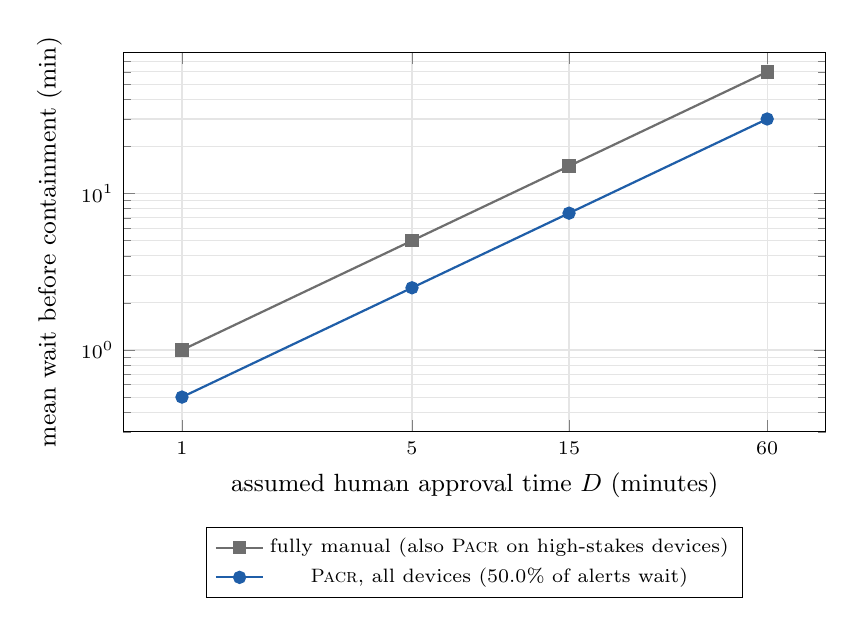
\begin{tikzpicture}
\begin{axis}[
  width=10.5cm, height=6.4cm, xlabel={assumed human approval time $D$ (minutes)}, ylabel={mean wait before containment (min)},
  xmode=log, ymode=log, xtick={1,5,15,60}, xticklabels={1,5,15,60}, ymin=0.3, ymax=80,
  legend style={font=\scriptsize, at={(0.5,-0.25)}, anchor=north},
  grid=both, grid style={gray!20}, tick label style={font=\scriptsize}, label style={font=\small}]
\addplot[color=pacrgrey, mark=square*, thick] coordinates {(1,1) (5,5) (15,15) (60,60)};
\addlegendentry{fully manual (also \pacr{} on high-stakes devices)}
\addplot[color=pacrblue, mark=*, thick] coordinates {(1,0.5) (5,2.5) (15,7.5) (60,30.0)};
\addlegendentry{\pacr{}, all devices (50.0\% of alerts wait)}
\end{axis}
\end{tikzpicture}
\caption{Modelled mean wait before containment against an assumed approval time (fixed playbook: 0, not drawn on the log axis). The shares of alerts that wait are measured; $D$ is assumed.}
\label{fig:wait}
\end{figure}

\subsection{Discussion}
\label{sec:compare-disc}
Three points follow from the comparisons. First, detection accuracy is no longer the differentiator on CICIoMT2024: the published detectors and ours are all high, and our remaining weaknesses (ARP spoofing, scans) show up only in per-class metrics. Second, the safety result comes from the structure of the system, not from model quality: the Policy Engine's registry-based rule produces the 0.00\% regardless of what the agents say, and the guards stop wrong agent output from reaching the Policy Engine's inputs. Third, the cost is real and visible: half of alerts wait for a person, and false alarms are still isolated at a rate that the calibrated gate only partly reduces. These are the trade-offs a hospital would have to accept or tune, and they are the questions a deployment study with real clinicians must answer.

%% ==========================================================================
\section{Conclusion}
\label{sec:conclusion}
This paper presented \pacr, a patient-aware framework that turns detection of attacks on medical devices into a safe and auditable response. Its novelty is the evaluated combination: a real detector, language-model agents treated as untrusted and corrected by deterministic guards, rule-based risk and policy engines that always place a human before severe actions on patient-dependent devices, and tamper-evident provenance on a real Fabric network. On the full CICIoMT2024 test split the detector reached 99.52\% accuracy, and the system took 0.00\% unsafe autonomous actions against 99.72\% for a fixed playbook. In fault-injected runs the guards removed every unsafe action and false closure, and every tested ledger tampering was detected. Limits remain: device context and agents were simulated, false alarms are still isolated in about 41\% of cases, and the ledger used one orderer. Future work will evaluate real language models on hospital device inventories with clinician approval studies, and will run the ledger on a multi-orderer network.

%% ==========================================================================
\begin{thebibliography}{99}
\small
\bibitem{naghib2025} A.~Naghib, F.~S. Gharehchopogh, A.~Zamanifar, A comprehensive and systematic literature review on intrusion detection systems in the internet of medical things: current status, challenges, and opportunities, Artificial Intelligence Review 58 (2025) 114. \href{https://doi.org/10.1007/s10462-024-11101-w}{doi:10.1007/s10462-024-11101-w}.

\bibitem{dadkhah2024} S.~Dadkhah, E.~C.~P. Neto, R.~Ferreira, R.~C. Molokwu, S.~Sadeghi, A.~A. Ghorbani, CICIoMT2024: Attack vectors in healthcare devices -- a multi-protocol dataset for assessing IoMT device security, Internet of Things 28 (2024). (Elsevier PII S2542660524002920.) % TODO: add article number / DOI from the publisher page.

\bibitem{akar2025} G.~Akar, S.~Sahmoud, M.~Onat, U.~Cavusoglu, E.~Malondo, L2D2: A novel LSTM model for multi-class intrusion detection systems in the era of IoMT, IEEE Access 13 (2025) 7002--7013. \href{https://doi.org/10.1109/ACCESS.2025.3526883}{doi:10.1109/ACCESS.2025.3526883}.

\bibitem{shaikh2025} J.~A. Shaikh, C.~Wang, M.~W.~U. Sima, M.~Arshad, M.~Owais, D.~S.~M. Hassan, R.~Alkanhel, M.~S.~A. Muthanna, A deep reinforcement learning-based robust intrusion detection system for securing IoMT healthcare networks, Frontiers in Medicine 12 (2025) 1524286. \href{https://doi.org/10.3389/fmed.2025.1524286}{doi:10.3389/fmed.2025.1524286}.

\bibitem{hafid2025} A.~Hafid, M.~Rahouti, M.~Aledhari, Optimizing intrusion detection in IoMT networks through interpretable and cost-aware machine learning, Mathematics 13~(10) (2025) 1574. \href{https://doi.org/10.3390/math13101574}{doi:10.3390/math13101574}.

\bibitem{lin2025} X.~Lin, J.~Zhang, G.~Deng, T.~Liu, T.~Zhang, Q.~Guo, R.~Chen, IRCopilot: Automated incident response with large language models, arXiv:2505.20945 (2025), preprint.

\bibitem{gao2026} Y.~Gao, K.~Hammar, T.~Li, In-context autonomous network incident response: An end-to-end large language model agent approach, arXiv:2602.13156 (2026), preprint.

\bibitem{hasnain2023} M.~Hasnain, F.~R. Albogamy, S.~S. Alamri, I.~Ghani, B.~Mehboob, The Hyperledger Fabric as a blockchain framework preserves the security of electronic health records, Frontiers in Public Health 11 (2023) 1272787. \href{https://doi.org/10.3389/fpubh.2023.1272787}{doi:10.3389/fpubh.2023.1272787}.

\bibitem{pelekoudas2023} F.~Pelekoudas-Oikonomou, J.~C. Ribeiro, G.~Mantas, G.~Sakellari, J.~Gonzalez, Prototyping a Hyperledger Fabric-based security architecture for IoMT-based health monitoring systems, Future Internet 15~(9) (2023) 308. \href{https://doi.org/10.3390/fi15090308}{doi:10.3390/fi15090308}.

\bibitem{vidhya2023} S.~Vidhya, V.~Kalaivani, A blockchain based secure and privacy aware medical data sharing using smart contract and encryption scheme, Peer-to-Peer Networking and Applications (2023). \href{https://doi.org/10.1007/s12083-023-01449-1}{doi:10.1007/s12083-023-01449-1}. % TODO: add volume/pages

\bibitem{mukhopadhyay2021} A.~Mukhopadhyay, R.~Vinayaka, A smart-contract-based blockchain for a healthcare IoT network, International Journal of Electronic Healthcare (2021). \href{https://doi.org/10.1504/IJEH.2021.117122}{doi:10.1504/IJEH.2021.117122}. % TODO: add volume/pages

\bibitem{pranav2026} M.~M. Pranav, S.~Rithan, R.~D.~A. Raj, A.~Pallakonda, R.~M.~R. Yanamala, K.~Prakasha~K., Smart grid cybersecurity against power system MiTM threats and machine learning-based attack classification, Energy Reports (2026). \href{https://doi.org/10.1016/j.egyr.2025.12.035}{doi:10.1016/j.egyr.2025.12.035}. % TODO: add volume/article number

\bibitem{vignes2025} V.~M. Vignes, M.~P. Sri~Harini, R.~Satheesh, V.~Das, S.~Padmanaban, AI-driven cybersecurity framework for anomaly detection in power systems, Scientific Reports (2025). \href{https://doi.org/10.1038/s41598-025-19634-y}{doi:10.1038/s41598-025-19634-y}. % TODO: add volume/article number

\bibitem{alsolami2024} T.~Alsolami, B.~Alsharif, M.~Ilyas, Enhancing cybersecurity in healthcare: Evaluating ensemble learning models for intrusion detection in the Internet of Medical Things, Sensors 24~(18) (2024) 5937. \href{https://doi.org/10.3390/s24185937}{doi:10.3390/s24185937}.

\bibitem{abdelhaq2026} M.~Abdelhaq, S.~Palanisamy, M.~Gopinath, V.~G.~S. Manasa, M.~A. Ram, S.~Khan, et~al., A hybrid XGBoost--SVM ensemble framework for robust cyber-attack detection in the internet of medical things (IoMT), Scientific Reports 16 (2026) 6855. \href{https://doi.org/10.1038/s41598-026-37832-0}{doi:10.1038/s41598-026-37832-0}. % VERIFY the full author list

\bibitem{xiao2024} N.~Xiao, Z.~Wang, X.~Sun, J.~Miao, A novel blockchain-based digital forensics framework for preserving evidence and enabling investigation in industrial Internet of Things, Alexandria Engineering Journal 86 (2024) 631--643. % TODO: add DOI

\end{thebibliography}

\end{document}
